Við höfum kynnst því hvernig búa má til töflur (kafli \ref{kafli:uppsetningtaflna}) og hvernig ná má í gögn úr töflunum (kafli \ref{kafli:select}). 

Þessi vitneskja getur komið okkur furðu langt - en ekki alveg nógu langt. Nú skulum við skoða hvernig vinna má með stærri töflur og margar töflur í sama grunninum.
\section{Lyklar}
\label{undirkafli:lyklar}
Lyklar\footnote{e. \emph{key} eða \emph{index}} eru mikilvægir í öllum skilvirkum gagnagrunnum. Lyklar eru m.a. notaðir til að gera fyrirspurnir hraðvirkari og til að tengja töflur saman.

Lyklar eru stundum kallaðir \emph{vísar}. ``Lykill'' og ``vísir'' þýða það sama þegar kemur að MySQL.
\subsection{Almennt um lykla - KEY/INDEX}
Ímyndum okkur að við séum að leita að bók sem geymd er á mjög frumstæðu bókasafni. Á þessu bókasafni eru nefnilega engir titlar á kili bókanna og allar bækurnar líta eins út.
Erfitt verk, ekki satt? Að meðaltali þyrftum við að fara í gegnum hálft bókasafnið áður en við rekumst á bókina sem við viljum.

Þetta er verkið sem stendur frammi fyrir gagnagrunnskerfum í hvert skipti sem við notum þau til að leita að gögnum í dálki sem ekki er með lykil.
Gagnagrunnskerfi geta ekki borið saman gögn án þess að lesa þau.
Sem betur fer eru tölvur mjög fljótar að bryðja sér leið í gegn um mikið magn af gögnum - en við getum gert betur en að geyma allar upplýsingarnar okkar ómerktar og óraðar.

Það að setja vísi á dálk í gagnagrunnstöflu samsvarar því að búa til bókasafnskerfi sem getur sagt okkur í hvaða hillum og hvar í hillunum við getum fundið hverja bók. Það gefur auga leið að þetta gerir leitina auðveldari.

Hver tafla getur haft marga lykla.
\subsection{Einkvæmir lyklar - UNIQUE KEY}
Hægt er að setja þá takmörkun á lykil að öll stök sem honum tilheyra þurfi að vera einstök.

Slíkur lykill, sem kalla má einkvæman lykil\footnote{e. \emph{unique key} eða \emph{unique index}}, hefur þá ekki einungis það hlutverk að gera leit í gagnagrunninum auðveldari, heldur einnig það hlutverk að passa upp á að gögnin séu einstök.

Þetta þýðir að það að reyna að setja inn endurtekin gögn í dálk (dálka) sem er með einkvæman lykil veldur villu. Einkvæmur lykill myndar sem sagt takmörkun á því hvaða gildi mega fara inn í dálka sem hann nær yfir. Talað er um að einkvæmir lyklar myndi skorðu\footnote{e. \emph{constraint}} á dálkinn eða dálkana.

Íslenskar kennitölur eru dæmi um gögn sem oft væri gott að vera með einkvæman lykil á. Það að fletta upp kennitölum er algeng aðgerð og við vitum að allar kennitölur eiga að vera einstakar.
\subsection{Aðallyklar - PRIMARY KEY}
\label{undirkafli:adallyklar}
Við höfum kynnst aðallyklum áður. Við sáum útskýringu á hvernig búa má til slíkan lykil í undirkafla \ref{undirkafli:adallyklar-kynning}.

Nú getum við séð að aðallykill er ekkert annað en sérstök gerð af einkvæmum lykli. Aðallykill er lykill sem hefur það sérstaka hlutverk að einkenna hverja línu fyrir sig, svo að hægt sé að vísa í hana á ótvíræðan hátt.

Þar sem að aðallykill töflu á að geta einkennt hverja línu er oftast best að lykillinn sé ekki byggður á gögnunum í línunni \footnote{af því að við viljum alls ekki þurfa að breyta aðallykli línu ef að gögnin breytast}. Einnig er gott að aðallykillinn sé lítill og einfaldur\footnote{Vegna þess að hann er oftast mikið notaður af gagnagrunnskerfinu.}. 

Kennitölur eru þess vegna ekki sérstaklega góðir aðallyklar. Þær geyma upplýsingar um einstaklinginn (fæðingardagsetningu hans), þær geta breyst (þó það sé sjaldgæft) og þær eru langar (sem er tímafrekt að lesa). Þess vegna eru romsur á borð við þá sem við höfum séð í \verb|CREATE TABLE| skipunum, \verb|id INTEGER NOT NULL PRIMARY KEY AUTO_INCREMENT| mikið notaðar til að skilgreina aðallykla. Þær búa til lykla sem 
\begin{itemize}
 \item Auðkenna línuna fullkomlega
 \item Eru heiltölur (og þar með litlar og auðveldar í vinnslu)
 \item Eru aldrei \verb|NULL|
 \item Og eru óháðir gögnunum.
\end{itemize}
Þó að tafla geti verið með marga lykla, þá er hver tafla aðeins með einn aðallykil.

\begin{example}
\caption[PRIMARY KEY]{Til upprifjunar: aðallykill skilgreindur sem hluti af \emph{CREATE TABLE} skipun. Þessi skipun býr til töflu \ref{tafla:nemendur}, sem við notuðum mikið í síðasta kafla.}
\label{sql:k5d1-primary-key}
\centering
\sql{sql/k5d1-primary-key.sql}
\end{example}
\section{Margar töflur í sama gagnagrunninum}
Við komumst að því strax í kafla \ref{kafli:fyrstuskrefin} að gagnagrunnur getur innihaldið margar töflur. Hingað til höfum við samt verið að vinna með töflur eina í einu, óháð hvor annarri.

Lítum á dæmi um hvernig tvær töflur sem eru staddar í sama gagnagrunni geta tengst. Skoðum aftur áfangatöfluna okkar frá því í síðasta kafla (\ref{tafla:afangar-aftur}).

\begin{table}
\centering
\caption[Áfangar]{Tafla \ref{tafla:afangar} endurtekin.}
\label{tafla:afangar-aftur}
\begin{tabular}{llll}
\toprule
numer&audkenni&fag&onn\\
\midrule
1&	FOR1A3U&	Forritun&		1\\
2&	VSH1A3U&	Vefhönnun&		1\\
3&	GSÖ1G2U&	Notkun gagnasafna&	1\\
4&	TÆK1A1U&	Tölvutækni&		1\\
5&	FOR1B3U&	Forritun&		2\\
6&	VSH2A3U&	Vefhönnun&		2\\
7&	GSÖ1F2U&	Notkun gagnasafna&	2\\
8&	TÆK2A3U&	Tölvutækni&		2\\
9&	FOR2B2U&	Forritun&		3\\
10&	VSH2B2U&	Vefhönnun&		3\\
11&	GSÖ2B2U&	Notkun gagnasafna&	3\\
12&	TÆK2B2U&	Tölvutækni&		3\\
13&	GRU2L4U&	Lokaverkefni grunndeildar&3\\
\bottomrule
\end{tabular}
\end{table}

Sú tafla er ágæt, en við getum gert hana betri með því að skipta henni upp í tvær töflur sem eru tengdar saman.\footnote{Af hverju er betra að vera ekki með svona endurtekningar? Hér má til dæmis nefna minni plásseyðslu og hversu mikið auðveldara verður að uppfæra gildin í töflunum séu engar endurtekningar til staðar.} Tökum eftir því að nafnið á hverju fagi er endurtekið í dálkinum \emph{fag}. 

Við gætum komist hjá þessari endurtekningu með því að geyma nöfnin á fögunum í sérstakri töflu.\footnote{Það sem við erum að gera hér er kallað að ``normalísera'' (e. \emph{normalize}) gagnagrunninn. Normalísering er viðfangsefni fyrir lengra komna.} Sú tafla gæti verið eins og tafla \ref{tafla:fog}.
Þar má sjá að við höfum gefið hverju fagi númer. Gefum okkur það að dálkurinn sem inniheldur þau númer sé aðallykill (sjá undirkafla \ref{undirkafli:adallyklar}). Þá getum við notað númerin til þess að vísa í línurnar. Þetta hefur verið gert á töflu \ref{tafla:afangar-fagnumer}, nöfnunum á fögunum hefur verið skipt út fyrir númer þeirra í töflu \ref{tafla:fog}.

\begin{table}
\centering
\caption[Fög]{Fög, sem áður voru í gömlu áfangatöflunni (\ref{tafla:afangar}/\ref{tafla:afangar-aftur}). Þessa töflu má tengja við endurbættu áfangatöfluna - töflu \ref{tafla:afangar-fagnumer}.}
\label{tafla:fog}
\begin{tabular}{ll}
\toprule
numer&nafn\\
\midrule
1&Forritun\\
2&Vefhönnun\\
3&Notkun gagnasafna\\
4&Tölvutækni\\
5&Lokaverkefni grunndeildar\\
\bottomrule
\end{tabular}
\end{table}

\begin{table}
\centering
\caption[Áfangar - endurbætt]{Áfangataflan, þar sem nöfnunum á fögunum hefur verið skipt út fyrir númer þeirra, sem birtast í töflu \ref{tafla:fog}.}
\label{tafla:afangar-fagnumer}
\begin{tabular}{llll}
\toprule
numer&audkenni&fagNumer&onn\\
\midrule
1&	FOR1A3U&	1&	1\\
2&	VSH1A3U&	2&	1\\
3&	GSÖ1G2U&	3&	1\\
4&	TÆK1A1U&	4&	1\\
5&	FOR1B3U&	1&	2\\
6&	VSH2A3U&	2&	2\\
7&	GSÖ1F2U&	3&	2\\
8&	TÆK2A3U&	4&	2\\
9&	FOR2B2U&	1&	3\\
10&	VSH2B2U&	2&	3\\
11&	GSÖ2B2U&	3&	3\\
12&	TÆK2B2U&	4&	3\\
13&	GRU2L4U&	5&	3\\
\bottomrule
\end{tabular}
\end{table}

Hægt er að búa til mjög stórar fjölskyldur af töflum með því að tengja þær saman á þennan hátt með sameiginlegum gildum.

\begin{figure}
\caption[Tengsl taflna]{Sýnir hvernig töflur \ref{tafla:fog} og \ref{tafla:afangar-fagnumer} tengjast saman á dálkunum \emph{fagNumer} í áfangatöflunni og \emph{numer} í fagtöflunni. (Ath: Töflurnar eru ekki sýndar í heilu lagi.)}
\label{mynd:tengsl}
\centering
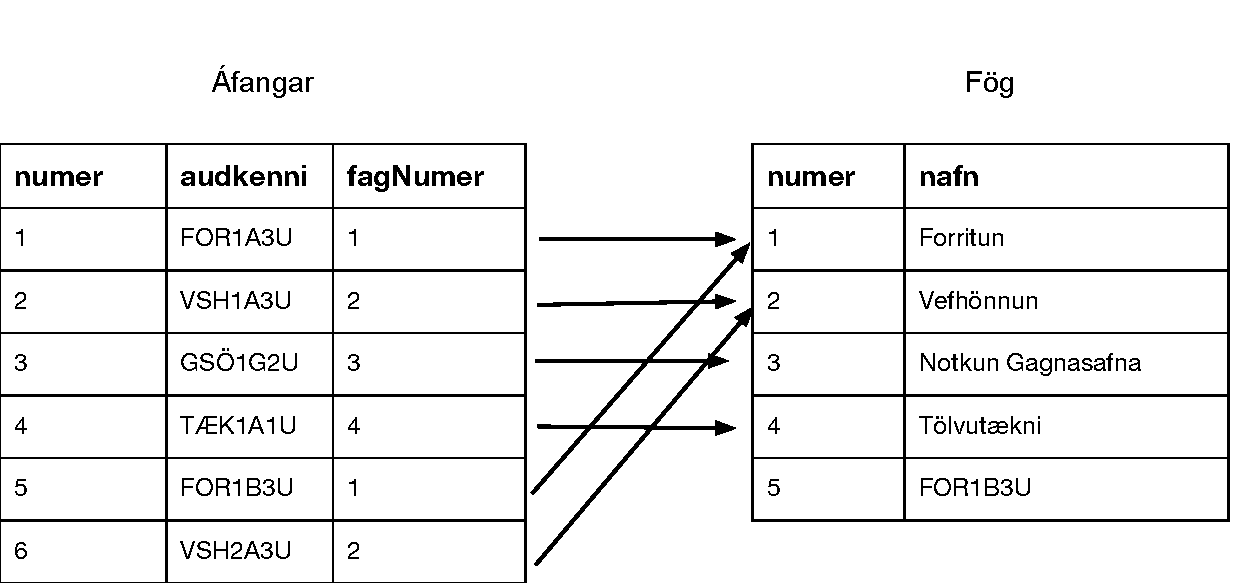
\includegraphics[width=\linewidth]{myndir/foreign-key}
\end{figure}

\section{Aðkomulyklar - FOREIGN KEY}
\label{undirkafli:adkomulyklar}
Þegar gildi í dálki eiga að vísa í línur annarrar töflu er hægt að tryggja sambandið með því að búa til svokallaðan aðkomulykil\footnote{e. \emph{Foreign key}.}.

Aðkomulykill myndar formlegt samband á milli tveggja taflna. Taflan sem inniheldur gögnin sjálf er kölluð foreldrið í sambandinu. Taflan sem inniheldur vísunina í gögnin er kölluð barnið\footnote{e. \emph{parent table} annars vegar og \emph{child table} hins vegar}. Í dæminu okkar á undan er \ref{tafla:fog} því foreldrið og \ref{tafla:afangar-fagnumer} barnið.

Aðkomulykillinn passar upp á að barnið geti ekki vísað í gögn sem ekki eru til í foreldrinu. Sé reynt að nota \verb|INSERT| skipun á barnið til að setja inn vísun í línu sem ekki er til í foreldrinu veldur það villu sé lykillinn rétt upp settur.\footnote{Aðkomulyklar eru því önnur gerð af skorðu (constraint).}

Aðkomulykillinn er skilgreindur í \verb|CREATE TABLE| skipun barnsins.

Mikilvægt er að dálkarnir í barninu og foreldrinu passi saman m.t.t. gagnagerðar (\ref{undirkafli:gagnagerdir}). Oftast er tengt saman á heiltöludálkum (sem þurfa að vera af sömu stærð).

Dálkurinn í foreldrinu sem aðkomulykillinn vísar í þarf að hafa aðallykil eða einkvæman lykil. Væri svo ekki gæti gagnagrunnskerfið ekki verið visst um hvaða línu í foreldrinu vísunin í barninu ætti við.

Sjá má hvernig skilgreina mætti samband á milli taflna \ref{tafla:fog} og \ref{tafla:afangar-fagnumer} sem hluta af \verb|CREATE TABLE| skipunum á sýnidæmi \ref{sql:k5d2-tengdar-toflur}.

\begin{example}
\caption[FOREIGN KEY - tengdar töflur]{Tengdar töflur. Aðkomulykillinn er skilgreindur í síðustu línu seinni \emph{CREATE TABLE} skipunarinnar. Línan býr til aðkomulykil fyrir dálkinn \emph{fagNumer} sem vísar í dálkinn \emph{numer} í töflunni Fog.}
\label{sql:k5d2-tengdar-toflur}
\centering
\sql{sql/k5d2-tengdar-toflur.sql}
\end{example}

\begin{example}
\caption[FOREIGN KEY - abstract dæmi]{Meira ``abstract'' dæmi um tengdar töflur. Hér koma hlutverk taflanna og dálkanna fram sem heiti, til að sýna sambandið betur.}
\label{sql:k5d3-abstract-toflur}
\centering
\sql{sql/k5d3-abstract-toflur.sql}
\end{example}

\section{Margar samtengdar töflur}
Nú þegar við kunnum að tengja saman tvær töflur er ekkert sem hindrar okkur í að tengja saman eins margar töflur og við viljum.

Sýnidæmi \ref{sql:k5d4-starfsmenn-nemendur} til \ref{sql:k5d5-hopar} bæta töflum við gagnagrunninn ``taekniskolinn'' sem við bjuggum til fyrir löngu (sýnidæmi \ref{sql:k2d4-create-database}). Þær töflur passa við töflurnar sem búnar voru til í dæmi \ref{sql:k5d2-tengdar-toflur}.

\begin{example}
\caption[Starfsmenn og nemendur]{Okkar gömlu góðu starfsmanna- og nemendatöflur (töflur \ref{tafla:starfsmenn-ts} og \ref{tafla:nemendur}) uppfærðar til að vera tengdar saman. Hér höfum við bætt dálkinum \emph{umsjonarkennari} við nemendatöfluna, sem inniheldur vísun í starfsmannatöfluna. Hver nemandi hefur sem sagt einn starfsmann sem er umsjónarkennari viðkomandi nemanda.}
\label{sql:k5d4-starfsmenn-nemendur}
\centering
\sql{sql/k5d4-starfsmenn-nemendur.sql}
\end{example}

\begin{example}
\caption[Hópar]{Hver áfangi getur verið kenndur oftar en einu sinni á önn, nemendum er þá skipt upp í hópa. Hér er tafla sem geymt gæti upplýsingar um hópa. Hópur getur hér verið með nafn (í Tækniskólanum er þetta oftast bara tala) og hámarksfjölda nemenda sem eigin einkenni. Síðan vísum við í áfangatöfluna til að skrá upplýsingar um hvaða áfanga er hér verið að kenna, og starfsmannatöfluna til að skrá upplýsingar um hver kennir hópinn.}
\label{sql:k5d5-hopar}
\centering
\sql{sql/k5d5-hopar.sql}
\end{example}

Hér höfum við ekki farið yfir hvernig vinna má með gögn úr mörgum töflum (velja úr mörgum töflum í einu). Slík gagnavinnsla er viðfangsefni kafla \ref{kafli:gagnavinnslamargartoflur}.

\section{Tengingar} % 1-1, 1-N, N-N
Samtenging á töflum getur táknað þrjár gerðir af samböndum. Gerðirnar eru \emph{1-1 sambönd}, \emph{1-N sambönd} og \emph{N-N sambönd}. Lítum stuttlega á þær.

\subsection{1-N: Einn tengdur í marga}
Lítum fyrst á gerð $1-N$þ Kalla mætti þá sambandsgerð ``einn-í-marga''\footnote{e. \emph{one-to-many}} samband (táknið $N$ þýðir hér ``margir''). Þetta er sú gerð af samböndum/tengingum sem við sjáum oftast.

Skoðum dæmi \ref{sql:k5d2-tengdar-toflur} aftur, með það fyrir augum að hér sé verið að tengja ``einn-í-marga''.

Ef við greinum sambandið á milli taflanna tveggja aðeins, þá sjáum við að hver áfangi tilheyrir nákvæmlega einu fagi. Enginn áfangi tilheyrir tveimur fögum. Hins vegar getur hvert fag samanstaðið af mörgum áföngum. Öll sambönd á milli taflna þar sem hver lína í annarri töflunni getur tengst mörgum línum í hinni töflunni, en ekki öfugt, eru $1-N$ sambönd.

Í $1-N$ sambandi er aðkomulykillinn settur í ``margir'' töfluna - barnið í sambandinu.
\subsection{1-1: Einn tengdur í einn}
\begin{marginfigure}
\caption[Sambandsgerðir]{Tengingar í sambandsgerðunum þremur.}
\label{mynd:tengingar}
\centering
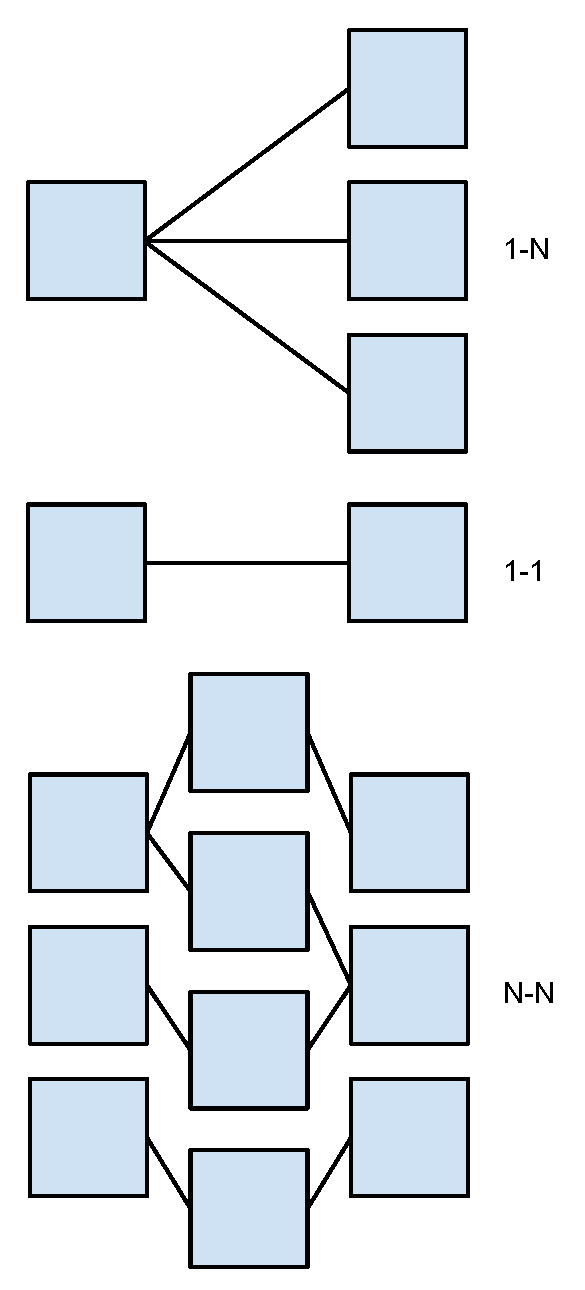
\includegraphics[width=\linewidth]{myndir/tengingar}
\end{marginfigure}
$1-1$ tengingar eru einfaldar tengingar. Við gætum kallað þær ``einn-í-einn'' tengingar. Ef $1-1$ tenging er á milli taflna samsvarar hver lína í annarri töflunni nákvæmlega einni línu í hinni töflunni, og öfugt.

Það að vera með $1-1$ tengingu á milli taflna er mjög svipað og að vera bara með eina töflu (hver lína í annarri töflunni er í raun bara framhald af línu í fyrri töflunni). Við sjáum þessa gerð tenginga oftast þegar gagnagrunnshönnuður sér að gott væri að skipta töflu með mörgum dálkum í nokkrar minni.

Í $1-1$ sambandi er aðkomulykill settur frá einum einkvæmum lykli til annars.
\subsection{N-N: Margir tengdir í marga}
Síðasta gerð tenginga er $N-N$ gerðin (``margir-í-marga'').

Til að sjá dæmi um hvernig $N-N$ tenging gæti komið upp getum við skoðað sambandið á milli hugtakanna ``nemendur'' og ``hópar'' (við bjuggum til töflur fyrir þessi hugtök í sýnidæmum \ref{sql:k5d4-starfsmenn-nemendur} og \ref{sql:k5d5-hopar}). Hver nemandi getur tilheyrt mörgum hópum. Hver hópur inniheldur meira en einn nemanda.

Ekki er hægt að tákna þetta samband með aðkomulyklum eingöngu svo vel sé. Til að tákna slík sambönd bætum við við sérstakri töflu. Þessi tafla, sem við getum kallað tengitöflu eða millitöflu, hefur það hlutverk að halda utan um sambandið. Hver lína í slíkri töflu táknar eitt samband.

Sýnidæmi \ref{sql:k5d6-hopskraning} sýnir hvernig búa mætti til tengitöflu sem skilgreinir $N-N$ samband á milli nemenda og hópa.

\begin{example}
\caption[Hópskráning: N-N]{Sambandið á milli hópa og nemenda táknað með tengitöflu. Taflan hefur tvo aðkomulykla. Hver lína í töflunni táknar eina skráningu nemanda í hóp.}
\label{sql:k5d6-hopskraning}
\centering
\sql{sql/k5d6-hopskraning.sql}
\end{example}

\section{Að sjá yfirlit gagnagrunns í MySQL Workbench}
Eftir því sem gagnagrunnar stækka verður erfiðara að átta sig á tengingunum á milli taflnanna sem honum tilheyra.

\begin{marginfigure}
\caption[Workbench - Reverse Engineer takki]{Reverse Engineer takkinn í MySQL Workbench.}
\label{mynd:reverse-engineer}
\centering
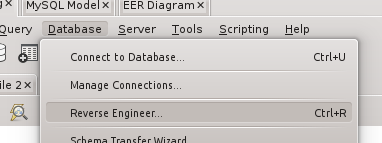
\includegraphics[width=\linewidth]{myndir/workbench-reverse-engineer}
\end{marginfigure}

MySQL Workbench getur sem betur fer aðstoðað okkur við að halda utan um gagnagrunna. Meðal annars getur hann búið til mynd af gagnagrunninum sem sýnir töflur gagnagrunnsins, dálka þeirra, lykla og sambönd.

Til að búa til slíka mynd út frá gagnagrunni sem þegar er til má velja valkostinn ``Reverse Engineer'' undir ``Database'' í aðalvalmynd MySQL Workbench (sjá mynd \ref{mynd:reverse-engineer}) eða ýta á \emph{CTRL+R} og fylgja leiðbeiningunum sem þar birtast. 

Útkoman verður lík mynd \ref{mynd:eer}.
\begin{figure}
\caption[Tækniskólagagnagrunnurinn]{Yfirlitsmynd fyrir Tækniskólagagnagrunninn, búin til af MySQL Workbench.}
\label{mynd:eer}
\centering
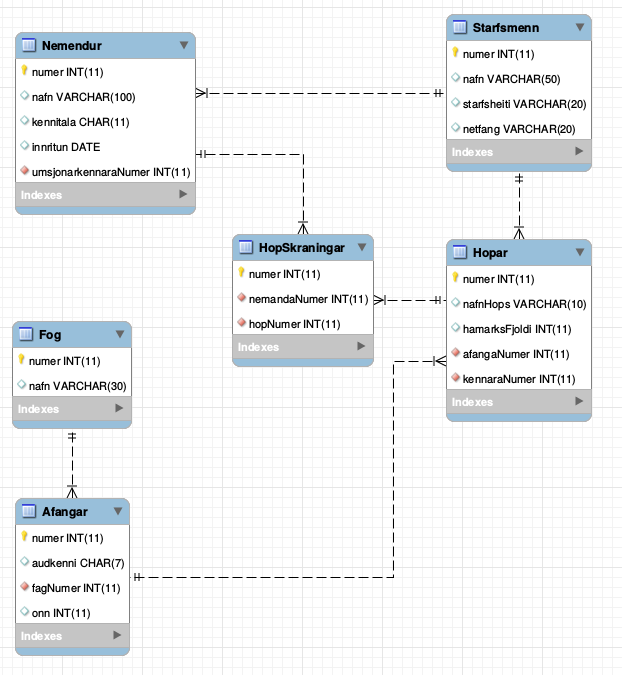
\includegraphics[width=\linewidth]{myndir/workbench-eer}
\end{figure}

\newpage
\section{(Ekki) meira um lykla}
Lyklar eru stórt viðfangsefni sem ekki er hægt að snerta á nema að mjög litlu leyti í þessari bók. Við munum ekki kafa dýpra í þá hér, heldur munum við láta þá bíða bóka og námskeiða fyrir lengra komna.
\section{Yfirlit}
Í þessum kafla skoðuðum við lykla og tengingar á milli taflna.

\begin{itemize}
 \item Það að setja lykil á dálk hjálpar gagnagrunnskerfi að vinna með hann á hagkvæman máta.
 \begin{itemize}
  \item Einn lykill getur náð yfir marga dálka.
  \item Hver tafla getur haft marga lykla.
 \end{itemize}
 \item Lykill getur verið ``einkvæmur'' (unique). Engin tvö stök í einkvæmum lykli eru eins.
 \item Hver tafla getur verið með einn aðallykil, sem er einkvæmur lykill. Hann er notaður til að auðkenna hverja línu í töflunni fyrir sig.
 \item Aðkomulykill er sérstök gerð af lykli sem skilgreinir samband á milli tveggja taflna.
 \item Aðkomulyklar og einkvæmir lyklar eru skorður (constraints). Villa kemur upp sé reynt að setja inn gögn í dálk sem tilheyrir slíkum lykli ef gögnin uppfylla ekki skilyrðin sem lykillinn setur.
 \item Sambönd á milli taflna geta verið á þrjá vegu: $1-N$, $1-1$ og $N-N$.
 \begin{itemize}
  \item Í $1-N$ sambandi er aðkomulykillinn í ``margir'' hluta sambandsins (barnið).
  \item Í $1-1$ sambandi tengir aðkomulykillinn saman tvo einkvæma lykla. 
  \item í $N-N$ sambandi eru tveir aðkomulyklar í sérstakri tengitöflu.
 \end{itemize}
 \item Hægt er að fá yfirlitsmynd af gagnagrunni með því að nota Reverse Engineer tólið í MySQL Workbench.
\end{itemize}





